\documentclass[onecolumn]{article}
\usepackage{graphicx} % Required for inserting images
\usepackage{amsmath}
\usepackage{amsfonts}
\usepackage{pythonhighlight}
\usepackage{datetime}
\usepackage{subcaption}
\usepackage{titling}
\usepackage{matlab-prettifier}
\usepackage{hyperref}
\usepackage[a4paper, total={6in, 8in}]{geometry}

\footskip = 1pt
\textheight = 700pt
\setlength{\droptitle}{-10em}

\title{IN3170 - Lab 2}
\author{Andreas Engøy, Erik Røset \& Daniel Tran}
\date{\monthname[\the\month] \the\year}

\begin{document}
\maketitle

\section{Introduction}
This lab rapport details the two tasks for Lab 2 in the course IN3170 Microelectronics. In the first task a double inverter circuit is built in order to probe, measure and calculate different characteristics of the circuit. In the second task [ONE SENTENCE DESCRIPTION OF TASK 2]

\section{Theory}
\subsection{Propagation delay}
The propagation delay of a logic gate e.g. Complementary Metal-Oxide-Semiconductor (CMOS) inverter is the time difference for the output signal as the input signal changes. It is usually measured at 50\% at the transition from input to output. The propagation delay is a measure of how fast the logic gate can respond to a change in the input signal.

\begin{figure}[h!]
    \centering
    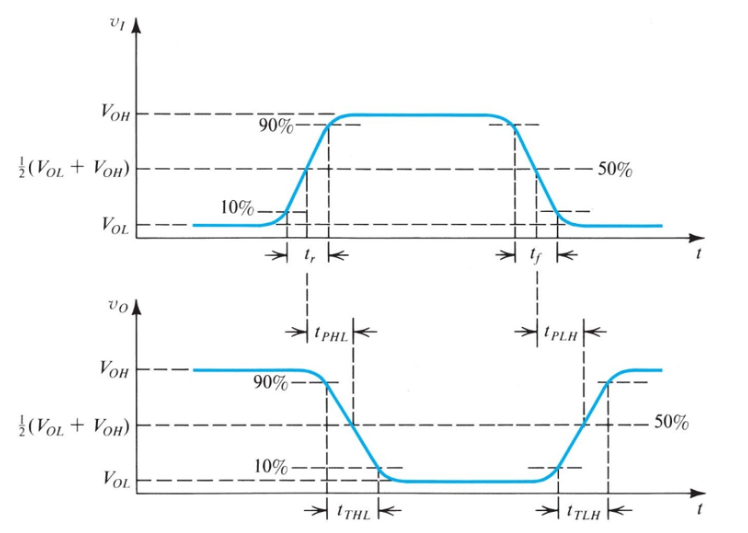
\includegraphics[width=0.6\textwidth]{tphl.png}
    \caption{Illustration of propagation delay and transition time of a logic gate. [Häfliger, 2018]}
    \label{fig:tphl}
\end{figure}

Figure \ref{fig:tphl} shows the different timing parameters for a logic gate. The propagation delay high-to-low $t_{pHL}$ and propagation delay low-to-high $t_{pLH}$ are the time it takes for the output to switch as input switches, measured from 50\% of the input signal to 50\% of the output signal. The rise time $t_{r}$ is the time it takes during transition for the output to switch from 10\% to 90\% of maximum output voltage. The fall time $t_{f}$ is the time it takes for the output to switch from 90\% to 10\% of maximum output voltage.

\subsection{RC circuit model of CMOS inverter}
The switching behavior of a CMOS inverter could be modeled as an first order RC network. The input capacitance of the inverter $C_I$ is charged or discharged through the resistor. The time constant $\tau$ of the circuit is given by the product of the resistance and the capacitance as given in the lab manual:
\begin{equation}\label{eq:tau} \tau = R_{on}C_{tot}\end{equation}
 where $R_{on}$ is the average resistance of the transistor when it is 'on' and $C_{tot}$ is the load capacitance.

\newpage

\section{Materials and Methods}
\subsection{Equipment}
\begin{table}[h!]
    \centering
    \begin{tabular}{|c|c|c|}
        \hline
        \textbf{Component} & \textbf{Model} & \textbf{Quantity} \\
        \hline
        Resistor & 100k$\Omega$ & 1 \\
        Hex Inverter IC & 74HCT14 & 1 \\
        Copper wires & - & 12 \\
        Printed Circuit Board & - & 1 \\
        Soldering iron & - & 1 \\
        Soldering wire & - & 1 \\
        Oscilloscope & HP54622 & 1 \\
        Waveform generator  & HP33120 & 1 \\
        Voltage source & HPE3631 & 1 \\ 
        \hline
    \end{tabular}
    \caption{List of components used in the experiment.}
    \label{tab:bom}
\end{table}

\subsection{Task 1a}

\begin{figure}[h!]
    \centering
    \begin{subfigure}{.5\textwidth}
      \centering
      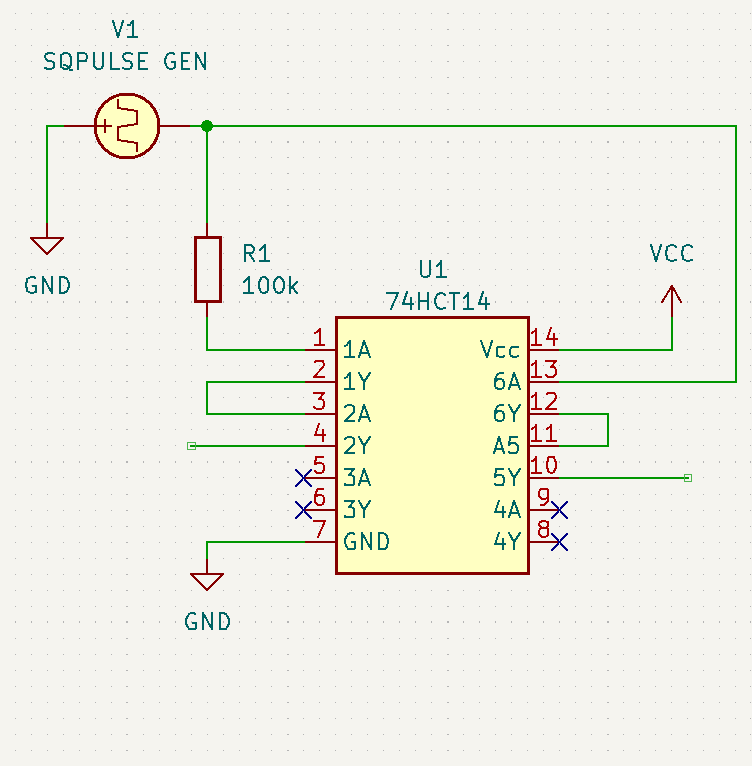
\includegraphics[width=.78\linewidth]{Task 1 Circuit.png}
      \caption{Circuit diagram}
      \label{fig:sub1}
    \end{subfigure}%
    \begin{subfigure}{.5\textwidth}
      \centering
      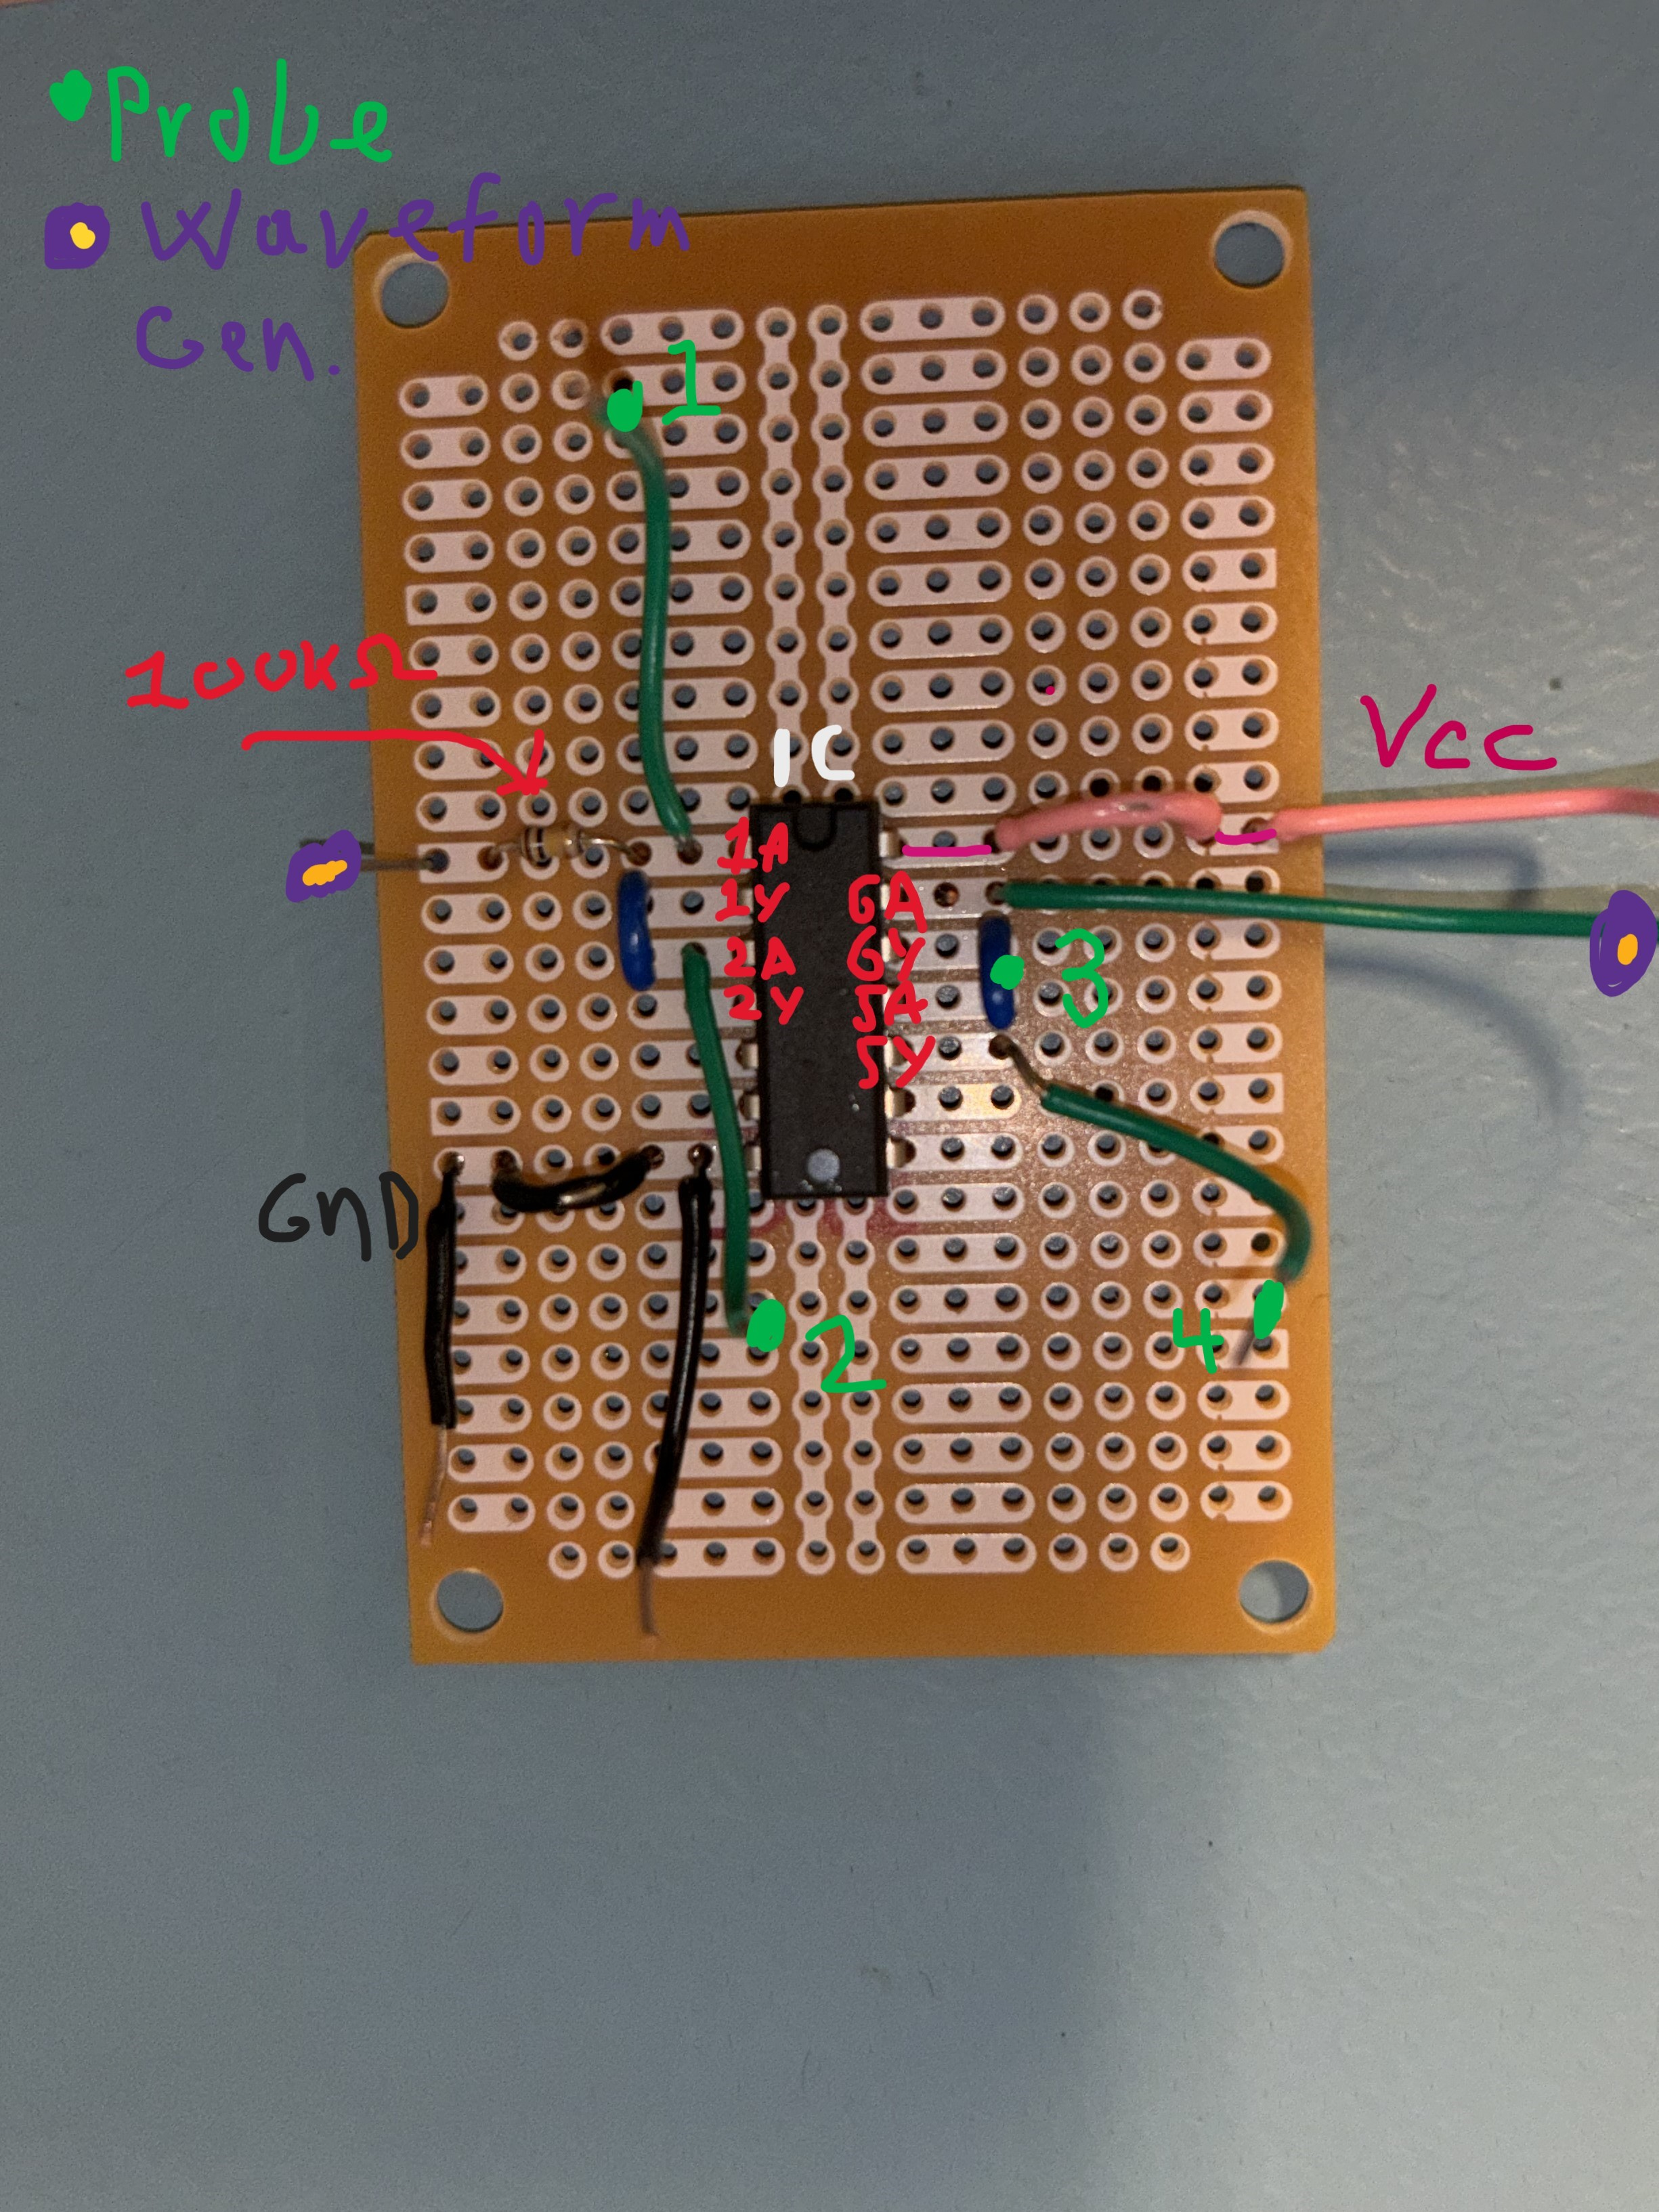
\includegraphics[width=.6\linewidth]{Photo of circuit 2.jpg}
      \caption{Photo of the circuit}
      \label{fig:sub2}
    \end{subfigure}
    \caption{Schematic and photo of two double inverters connected in series}
    \label{fig:1}
\end{figure}

The circuit is built according to the schematic in Figure \ref{fig:sub1}. The circuit has two separate double inverters, one with a 100k$\Omega$ resistor before the first inverter, and one without a resistor. The circuit is powered by a voltage source with a voltage of 5V. The probes of the circuit is connected to an oscilloscope in order to measure the voltage. The input marked 1A of the IC is connected to a waveform generator which generates a square wave with a frequency of 400 Hz. The circuit is then probed according to Figure 1 in the lab manual (point 1 in figure \ref{fig:sub2}).

Together with the lab manual there is supplied a Matlab script that controlls the settings of the waveform generator and the voltage source. It also reads the data from the oscilloscope and plots the data. From the given Matlab script the following modification were made:
\begin{itemize}
  \item The waveform generator was set to generate a square wave with a frequency of 400 Hz and peak voltage of 5 V on line 35 and 36.
  \item Autoscale for the oscilloscope was disabled on line 40.
  \item A system-specific dc offset was added to the oscilloscope to keep the signal within the 0 - 5 V range.
  \item The for-loop between lines 64 - 69 was swapped for a single line that set the voltage source to 5V.
  \item All plotting were modified to be labeled with correct axes and title.
\end{itemize}

In order to capture a single low-to-high transition, the oscilloscope display were manually adjusted as needed.
\begin{figure}[h!]
    \centering
    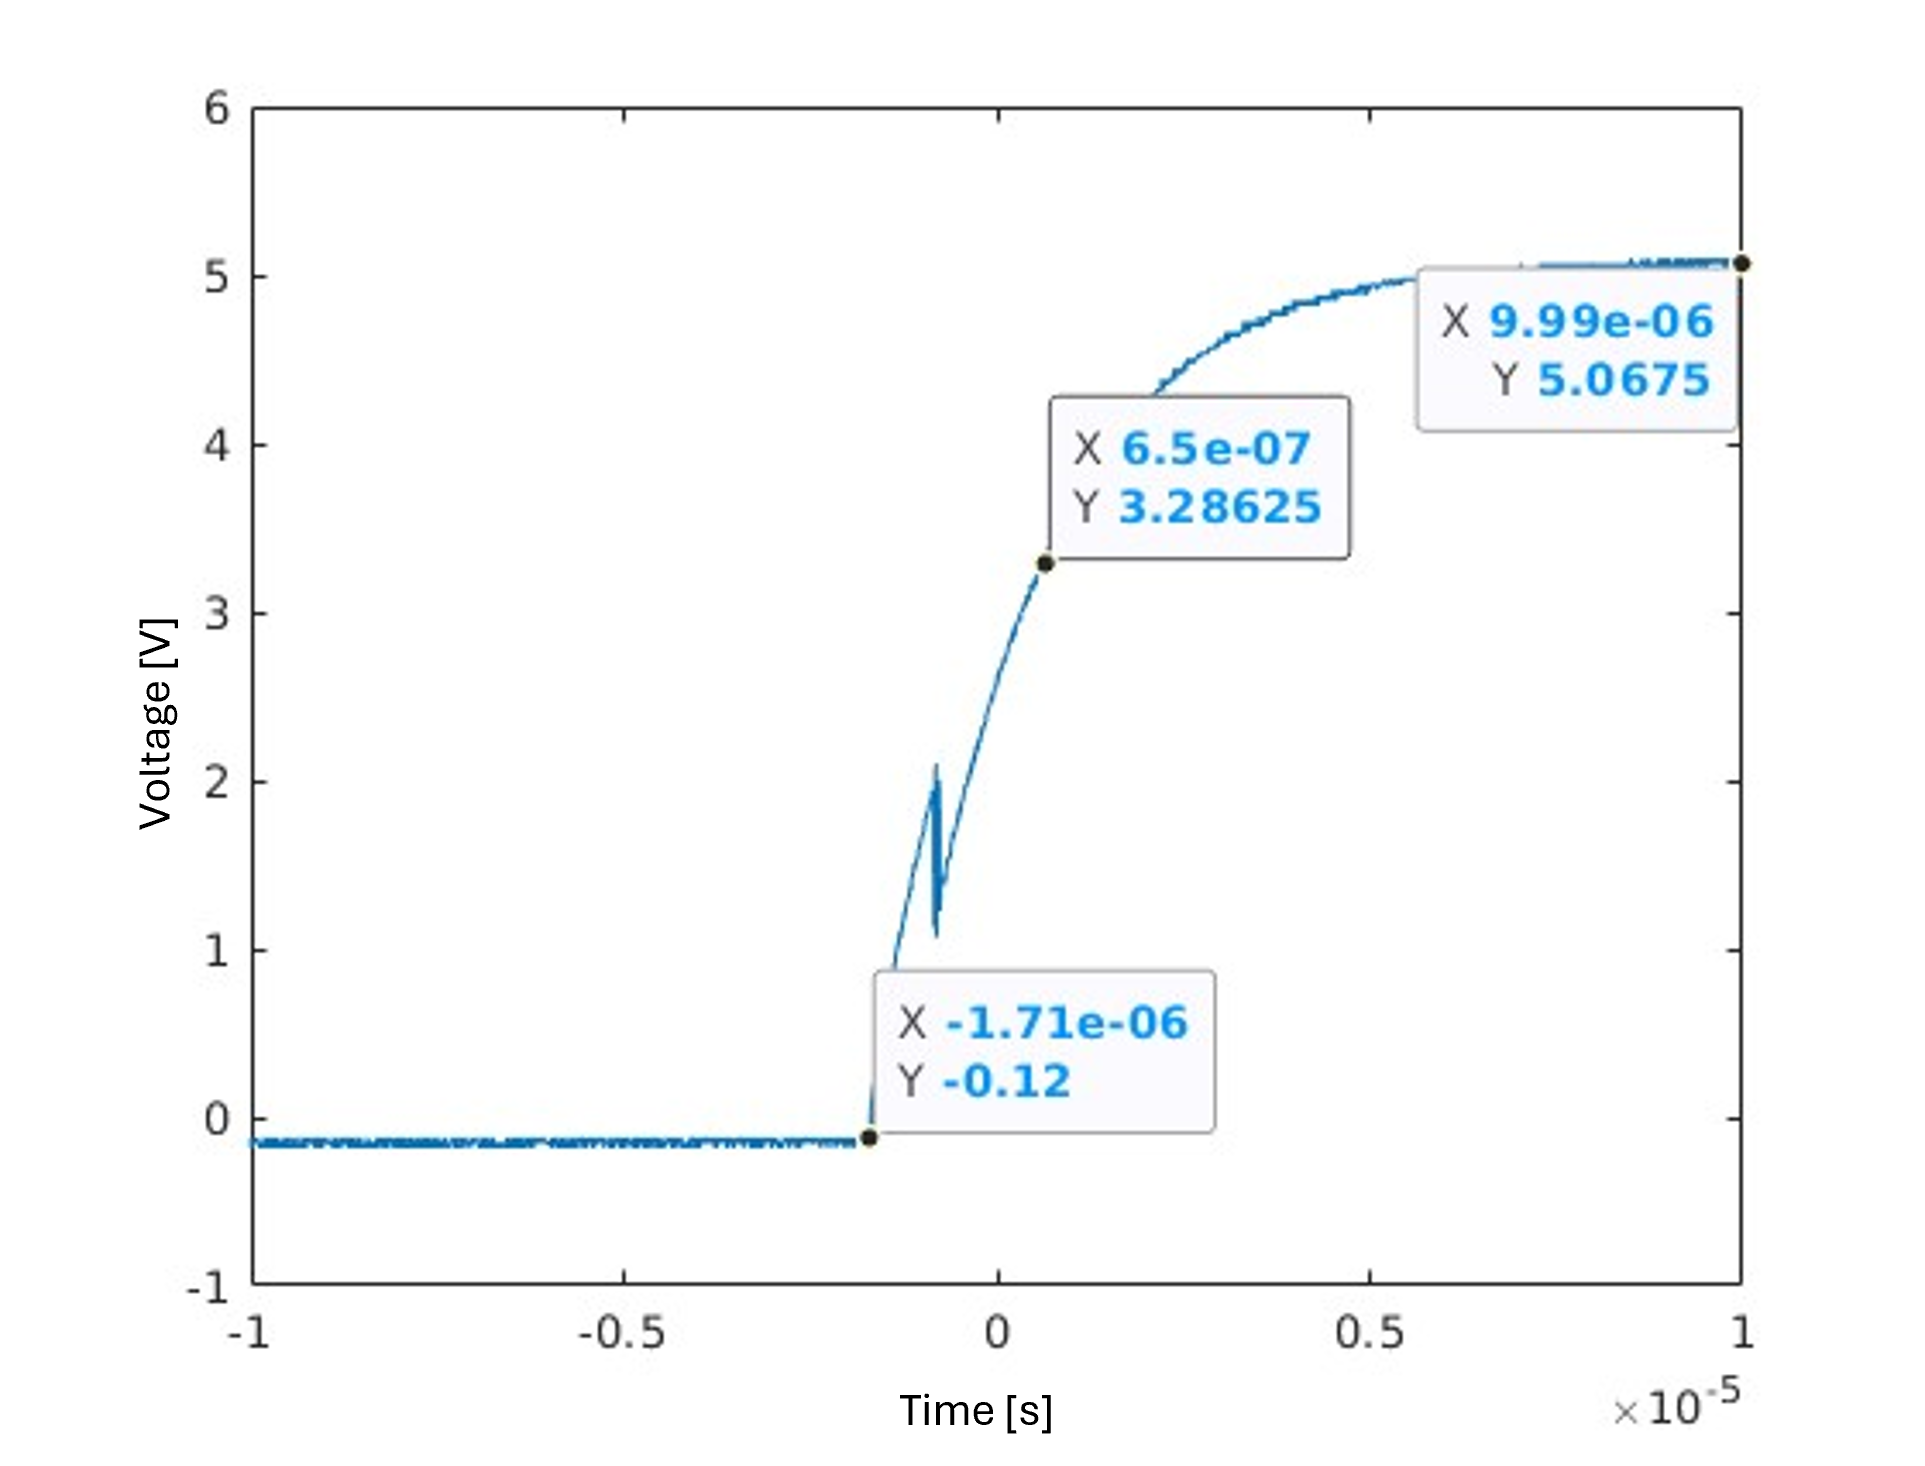
\includegraphics[width=0.6\textwidth]{plot1.png}
    \caption{Plot of the rising edge of a double inverter circuit with a 100k$\Omega$ resistor before the first inverter with added points of interest.}
    \label{fig:plot}
\end{figure}

From the plotted data, the start and end points of the rising edge were found together with the point of operation at Vdd/2. These were then used to find the input capacitance of the inverter using equation \ref{eq:tau}.

\subsection{Task 1b}
The wavegenerator is connected to input 6A of the IC. The probe measures the signal at point 3 from figure \ref{fig:sub2}. Another probe measures the output of the second inverter at point 4 from figure \ref{fig:sub2}. 

\begin{figure}[h!]
  \centering
  \begin{subfigure}{.5\textwidth}
    \centering
    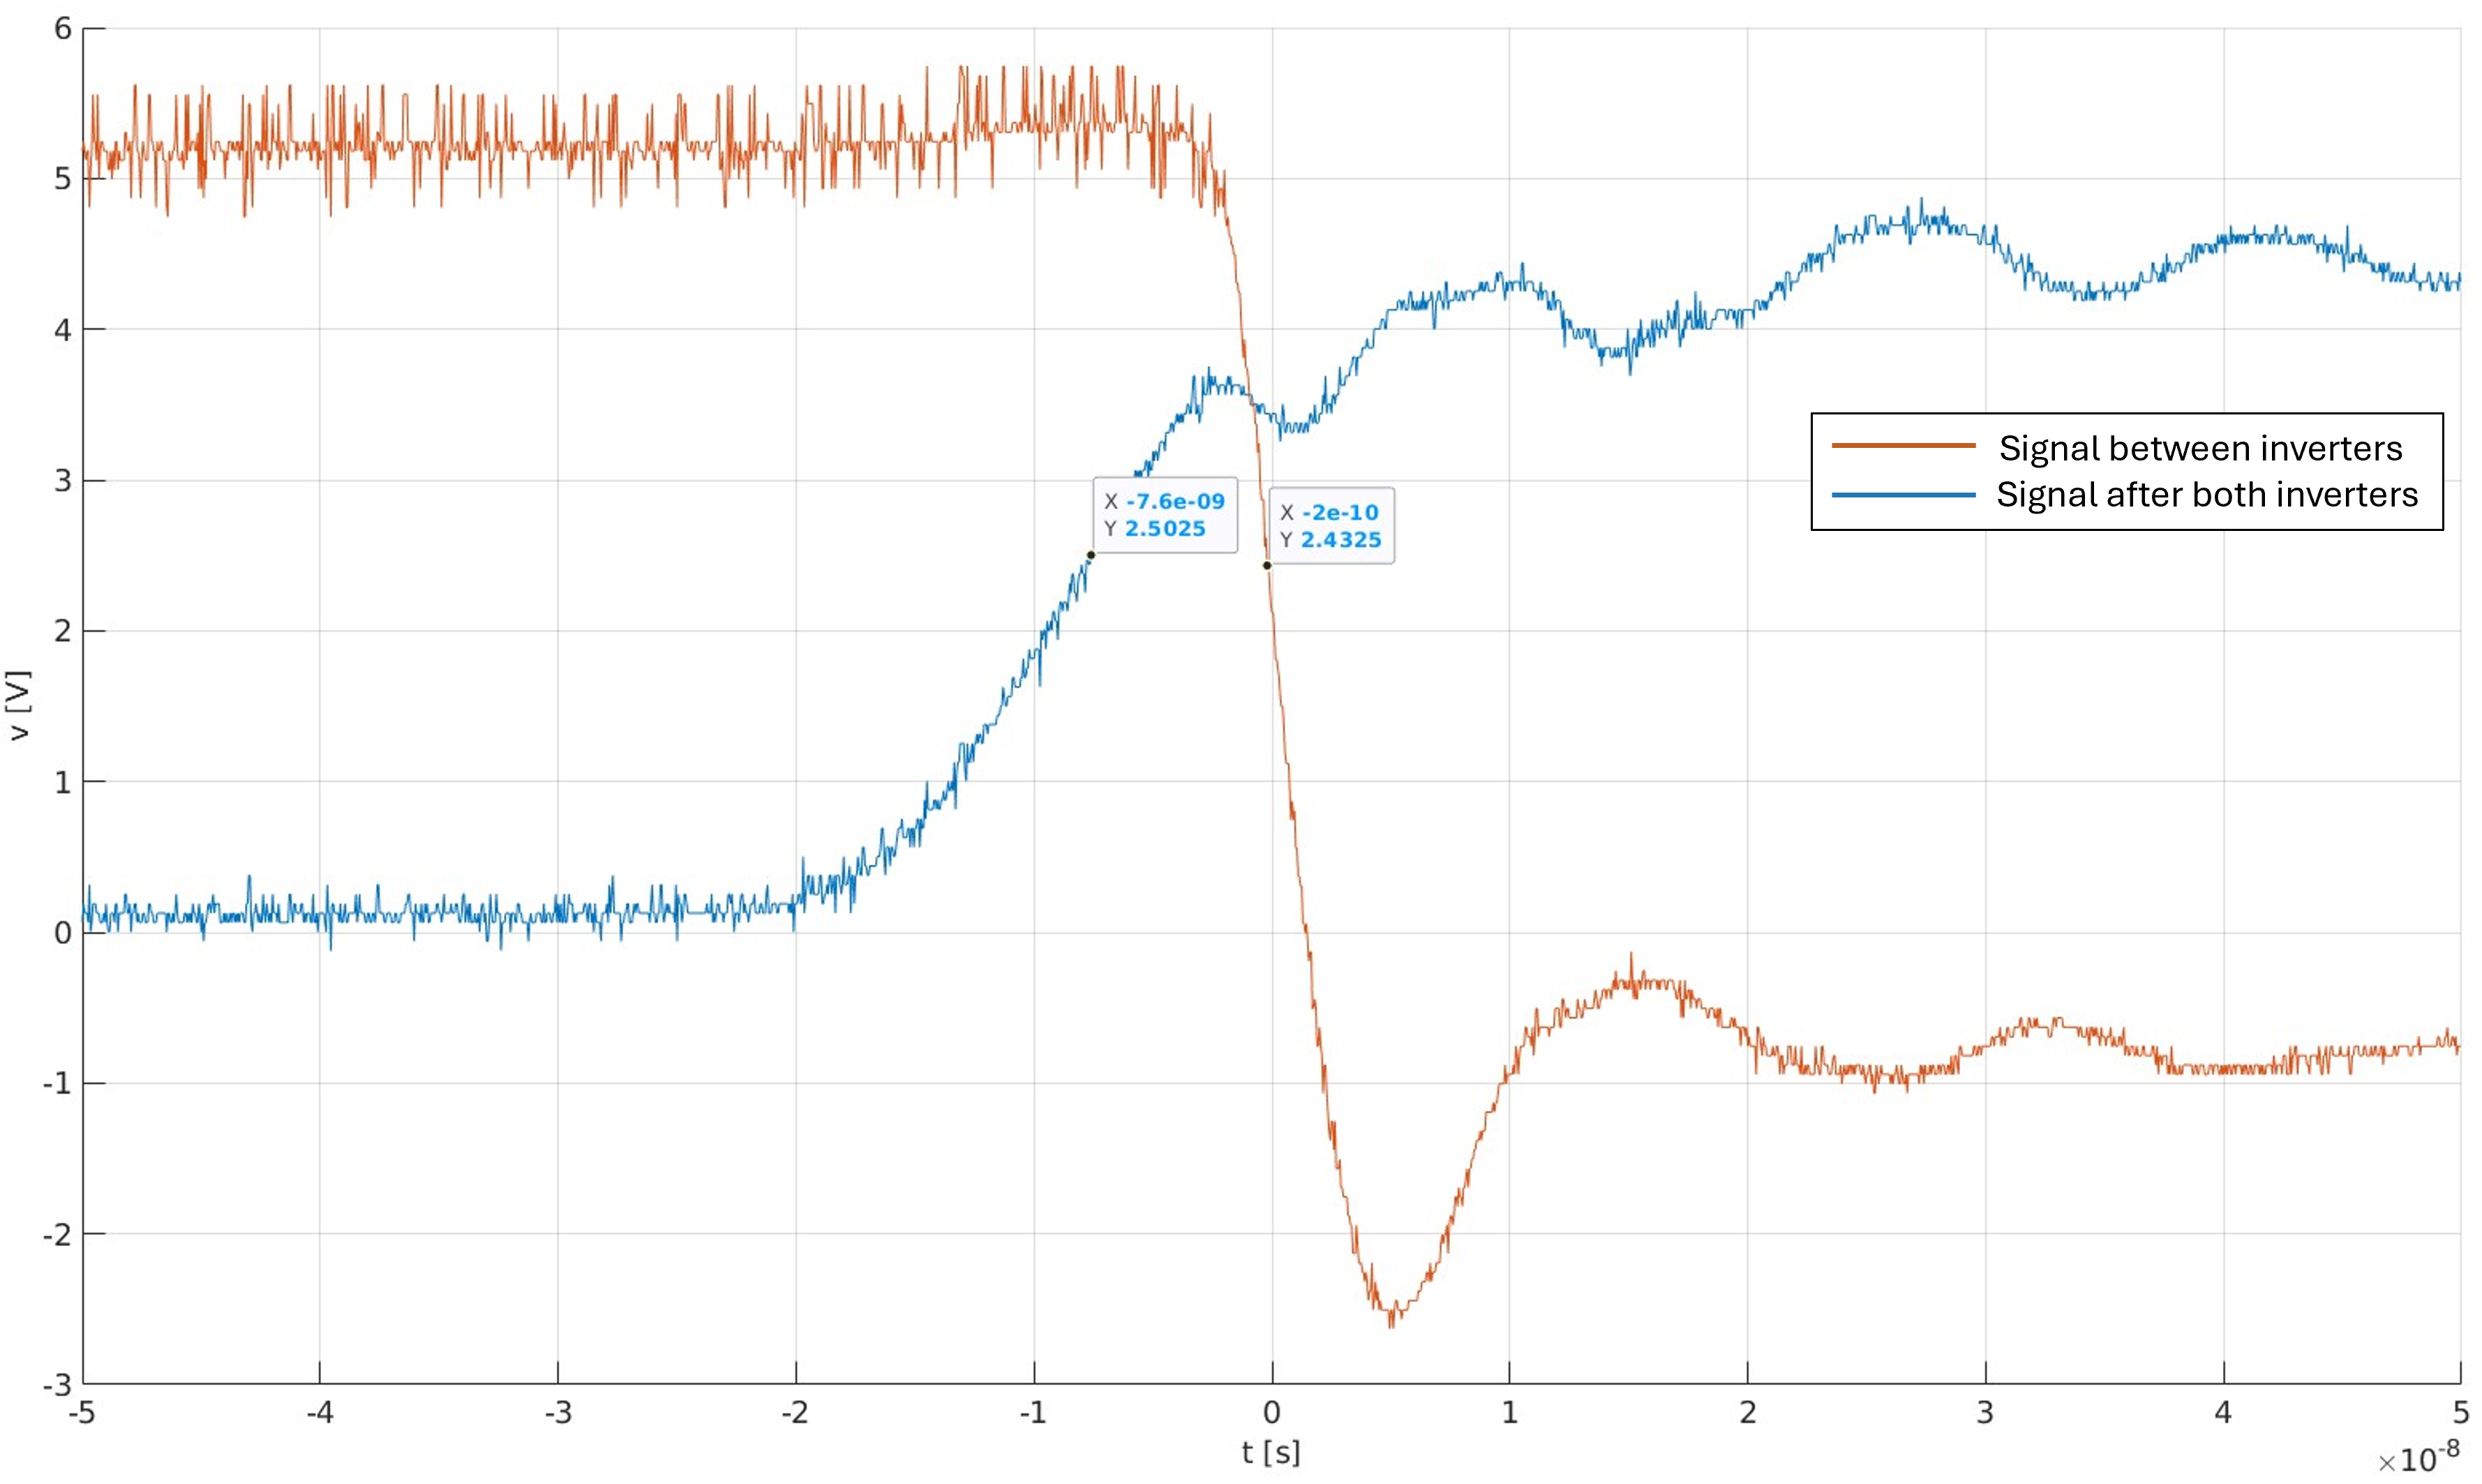
\includegraphics[width=.8\linewidth]{task2bhl2.png}
    \caption{High-to-low transition}
    \label{fig:sub3}
  \end{subfigure}%
  \begin{subfigure}{.5\textwidth}
    \centering
    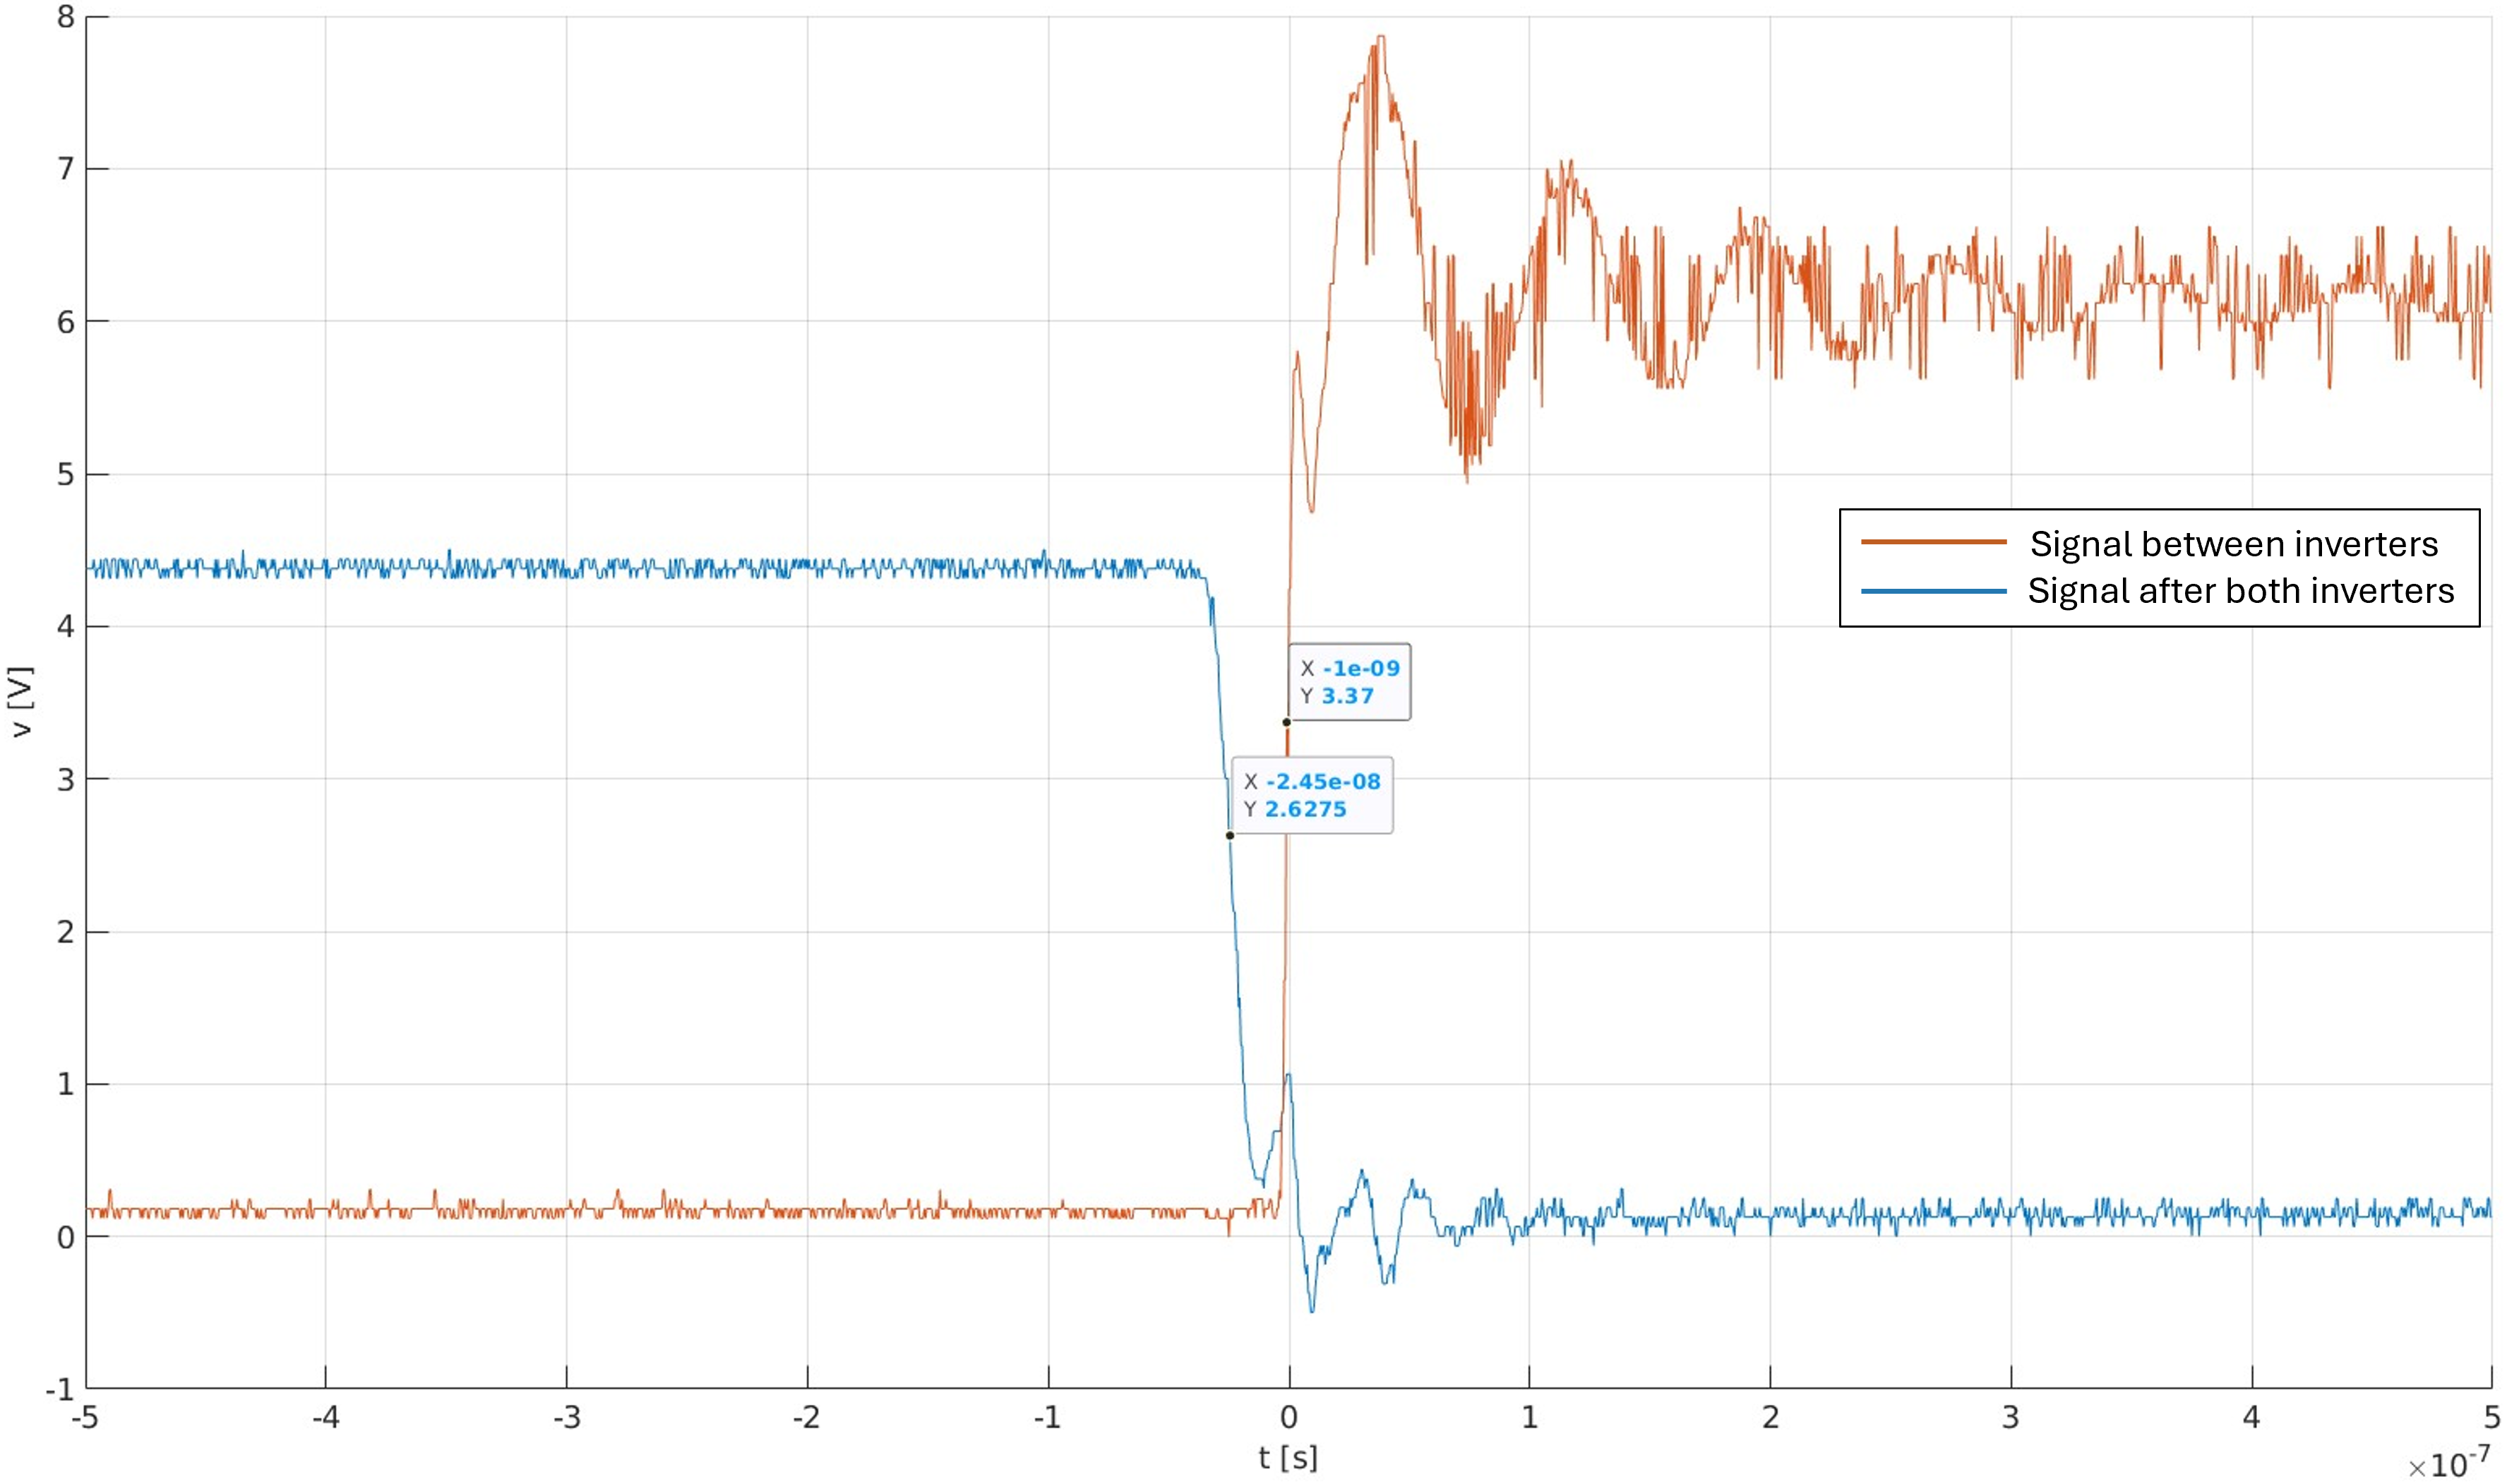
\includegraphics[width=.8\linewidth]{task2blh2.png}
    \caption{Low-to-high transition}
    \label{fig:sub4}
  \end{subfigure}
  \caption{Plots of the edges of a double inverter circuit without a resistor before the first inverter.}
  \label{fig:2}
\end{figure}


\section{Results}
\textbf{Input capacitance of the inverter:}
\begin{equation}
    C_{I} = 8.6 \ \text{pF}
\end{equation}




\section{Appendix}
\subsection{Calculations}
\textbf{Input capacitance of the inverter:}
From equation \ref{eq:tau} we use algebra to solve for $C_{I}$ with values from figure \ref{fig:plot}:
\begin{align}
    \tau &= R_{on}C_{tot} \nonumber \\
    \Rightarrow C_{tot} &= \frac{\tau}{R_{on}} \nonumber \\
    C_{I} + 15 \ \text{pF} &= \frac{\tau}{R_{on}} \nonumber \\
    C_{I} &= \frac{(6.5\cdot 10^{-7} \ \text{s}) - (-1.71 \cdot 10^{-6} \ \text{s})}{100 \ \text{k}\Omega} - 15 \ \text{pF}\nonumber \\
    C_{I} &= 8.6 \ \text{pF} \nonumber
\end{align}
Note: The lab manual states that 15 pF is to be subtracted from the total capacitance to get the input capacitance of the inverter. This is done to account for the capacitance of the oscilloscope probe.
\section{References}

Häfliger, P. (2018). Excerpt of Sedra/Smith Chapter 15: Inverter Delay [PDF]. University of Oslo. \url{https://www.uio.no/studier/emner/matnat/ifi/INF3410/h18/forelesningsfoiler/chapter15.pdf}
\end{document}